\section{Averaging models} \label{sec: average approach}
Because large scale word to word models seem to lack characteristics for a proper evaluation and interpretation of the results, the average approach was developed (\secreff{subsubsec: average approach}). The main idea is to rearrange the output of the formerly presented models, because general patterns like \texttt{Noun → Verb} or \texttt{Determiner → Adjective} appear significantly more frequently than certain instances as \texttt{sun → shines} or \texttt{an → old}. By averaging the predictions, one might be able to catch the structure in general.

Since \secreff{subsubsec: average approach} only provided a rough description of the principle, it shall be extended in the following. After the collective prediction of one word class, all outputs are averaged having one vector resembling the complete data in the dimension of the \cognitiveroom{} containing the associated frequencies. In the next step the $ n $ indices (in practice $ 10 $ was used) with the highest values are checked for their \postag{}. So, if index $ i $ is one of these and encodes the word \texttt{fish}, its \postag{} \ie \texttt{NOUN} is counted. Finally, a vector is constructed for all word classes where each component resembles the probability for the successor word class. Some final numbers are illustrated in \figref{\ref{fig: barplot det adp}}.

To get an idea of the learned results, some valid sentences are provided in German (the language of the training data of \figref{\ref{fig: barplot det adp}}) in \tabref{\ref{tab: example sentences}}. This short sanity check implies that no cacophony is learned and the outputs are reasonable.
\begin{figure}
	\centering
		\subcaptionbox{Averaged transitions of all \texttt{ADP}s compared to the ground truth.}{
			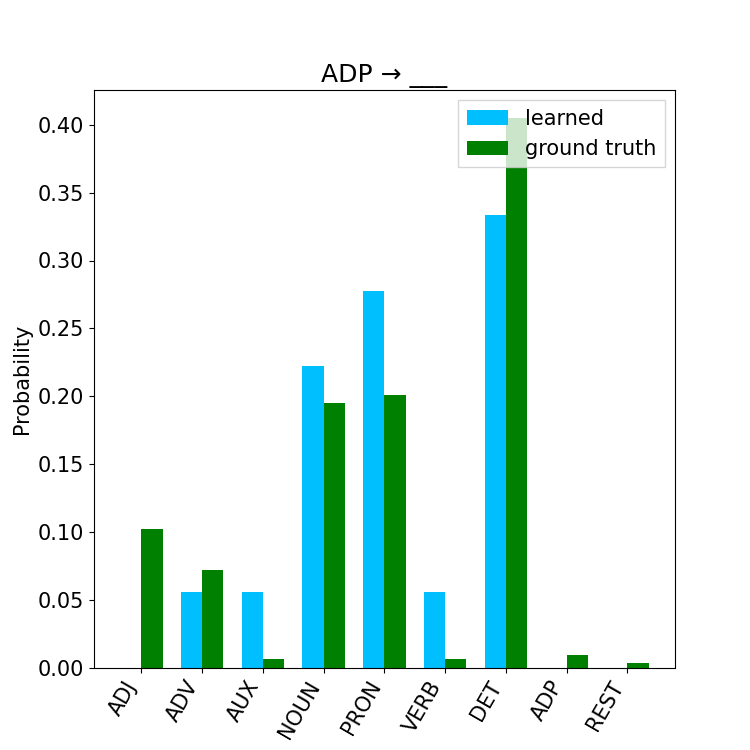
\includegraphics[width=\twocolpicwidth]{Bilder/chapter4/Barplots/Avg_OHE_OHE_5000E_100BS_1L_1C_200P_1500T_D/_epoch-4000//Combined_Barplot_ADP_S.png}
		}
		\hfill
		\subcaptionbox{Averaged transitions of all \texttt{ADJ}s compared to the ground truth.}{
			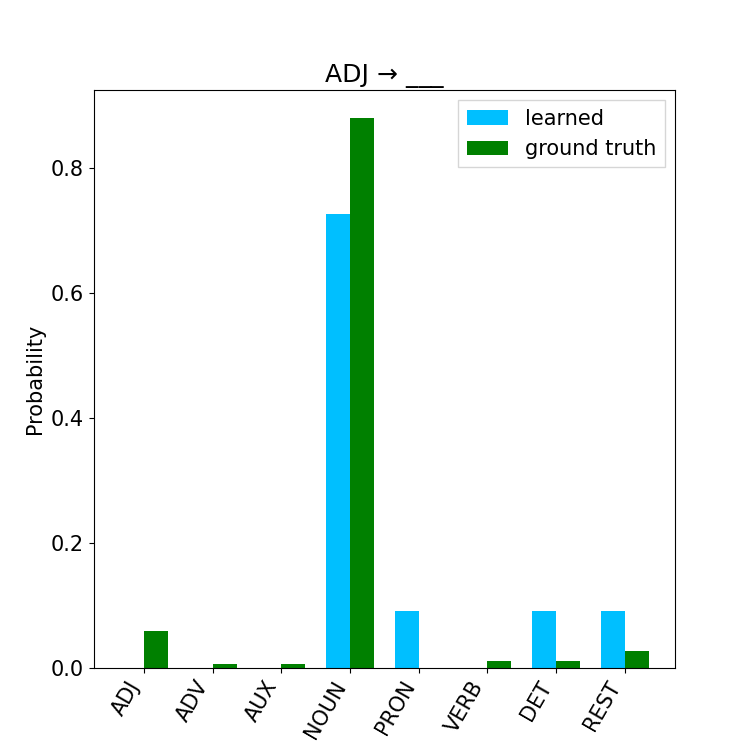
\includegraphics[width=\twocolpicwidth]{Bilder/chapter4/Barplots/Avg_OHE_OHE_5000E_100BS_1L_1C_200P_1500T_D/_epoch-4000//Combined_Barplot_ADJ_F.png}
		}
	\caption{Comparison of the averaged predictions (green) with the ground truth distribution (blue). The model was trained by \onehot{s} and german data. If a \postag{} has no blue bar, it has a $ 0 $\% probability to appear as successor \eg after an \texttt{ADJ} comes no \texttt{ADP}. The remaining plots of the other \postag{s} can be found in \appref{ch: appendix average approach}.}
	\label{fig: barplot det adp}
\end{figure}
\begin{table}
	\centering
	\caption[Schematic sentences for \postag{} rules]{Schematic sentences of the book used in \figref{\ref{fig: barplot det adp}}.}
	\begin{tabular}{l|l}
		\toprule
		Rule				& Sentence \\
		\midrule
		\texttt{ADP → NOUN}	& Sie hat mich \texttt{zum Schmunzeln}
		gebracht. \\
		\texttt{ADP → PRON}	& Es war überaus angenehm,
		sich \texttt{mit Ihnen} zu unterhalten. \\
		\texttt{ADP → DET}	& Ich bin nämlich eine gebürtige Linkshänderin,
		die \texttt{in der} Schule, [...] \\
		%%
		%		\texttt{DET → NOUN}	& \texttt{Das Werkzeug}, das im Keller liegt, [...] \\
		%		\texttt{DET → ADV}	& \texttt{Ein gut} ausgestattetes Museum, [...] \\
		%		\texttt{DET → ADP}	& Das Werkzeug, \texttt{das im} Keller liegt, [...] \\
		%
		\texttt{ADJ → NOUN}	& Lieber Leo, ich habe drei \texttt{fürchterliche Tage} hinter mir. \\
		\bottomrule
	\end{tabular}
	\label{tab: example sentences}
\end{table}

% --------------------------------------

\subsection{Averaging models: Evaluating the results}
The same configurations as in \secreff{subsec: text model evaluating the results} were processed. By ``configurations'' is subsumed: german and english, \onehot{} or word vector version and the same number of epochs and words used for training. After the unsatisfactory performance of the word vector approaches (\tabref{\ref{tab: text model versions and metrics}}), everything else than a similar outcome would be surprising. A detailed illustration of the results offers \figref{\ref{fig: rsme plots}}. By this plot it is also possible to talk about the outcomes a bit more specifically.
%
\begin{figure}
	\centering
		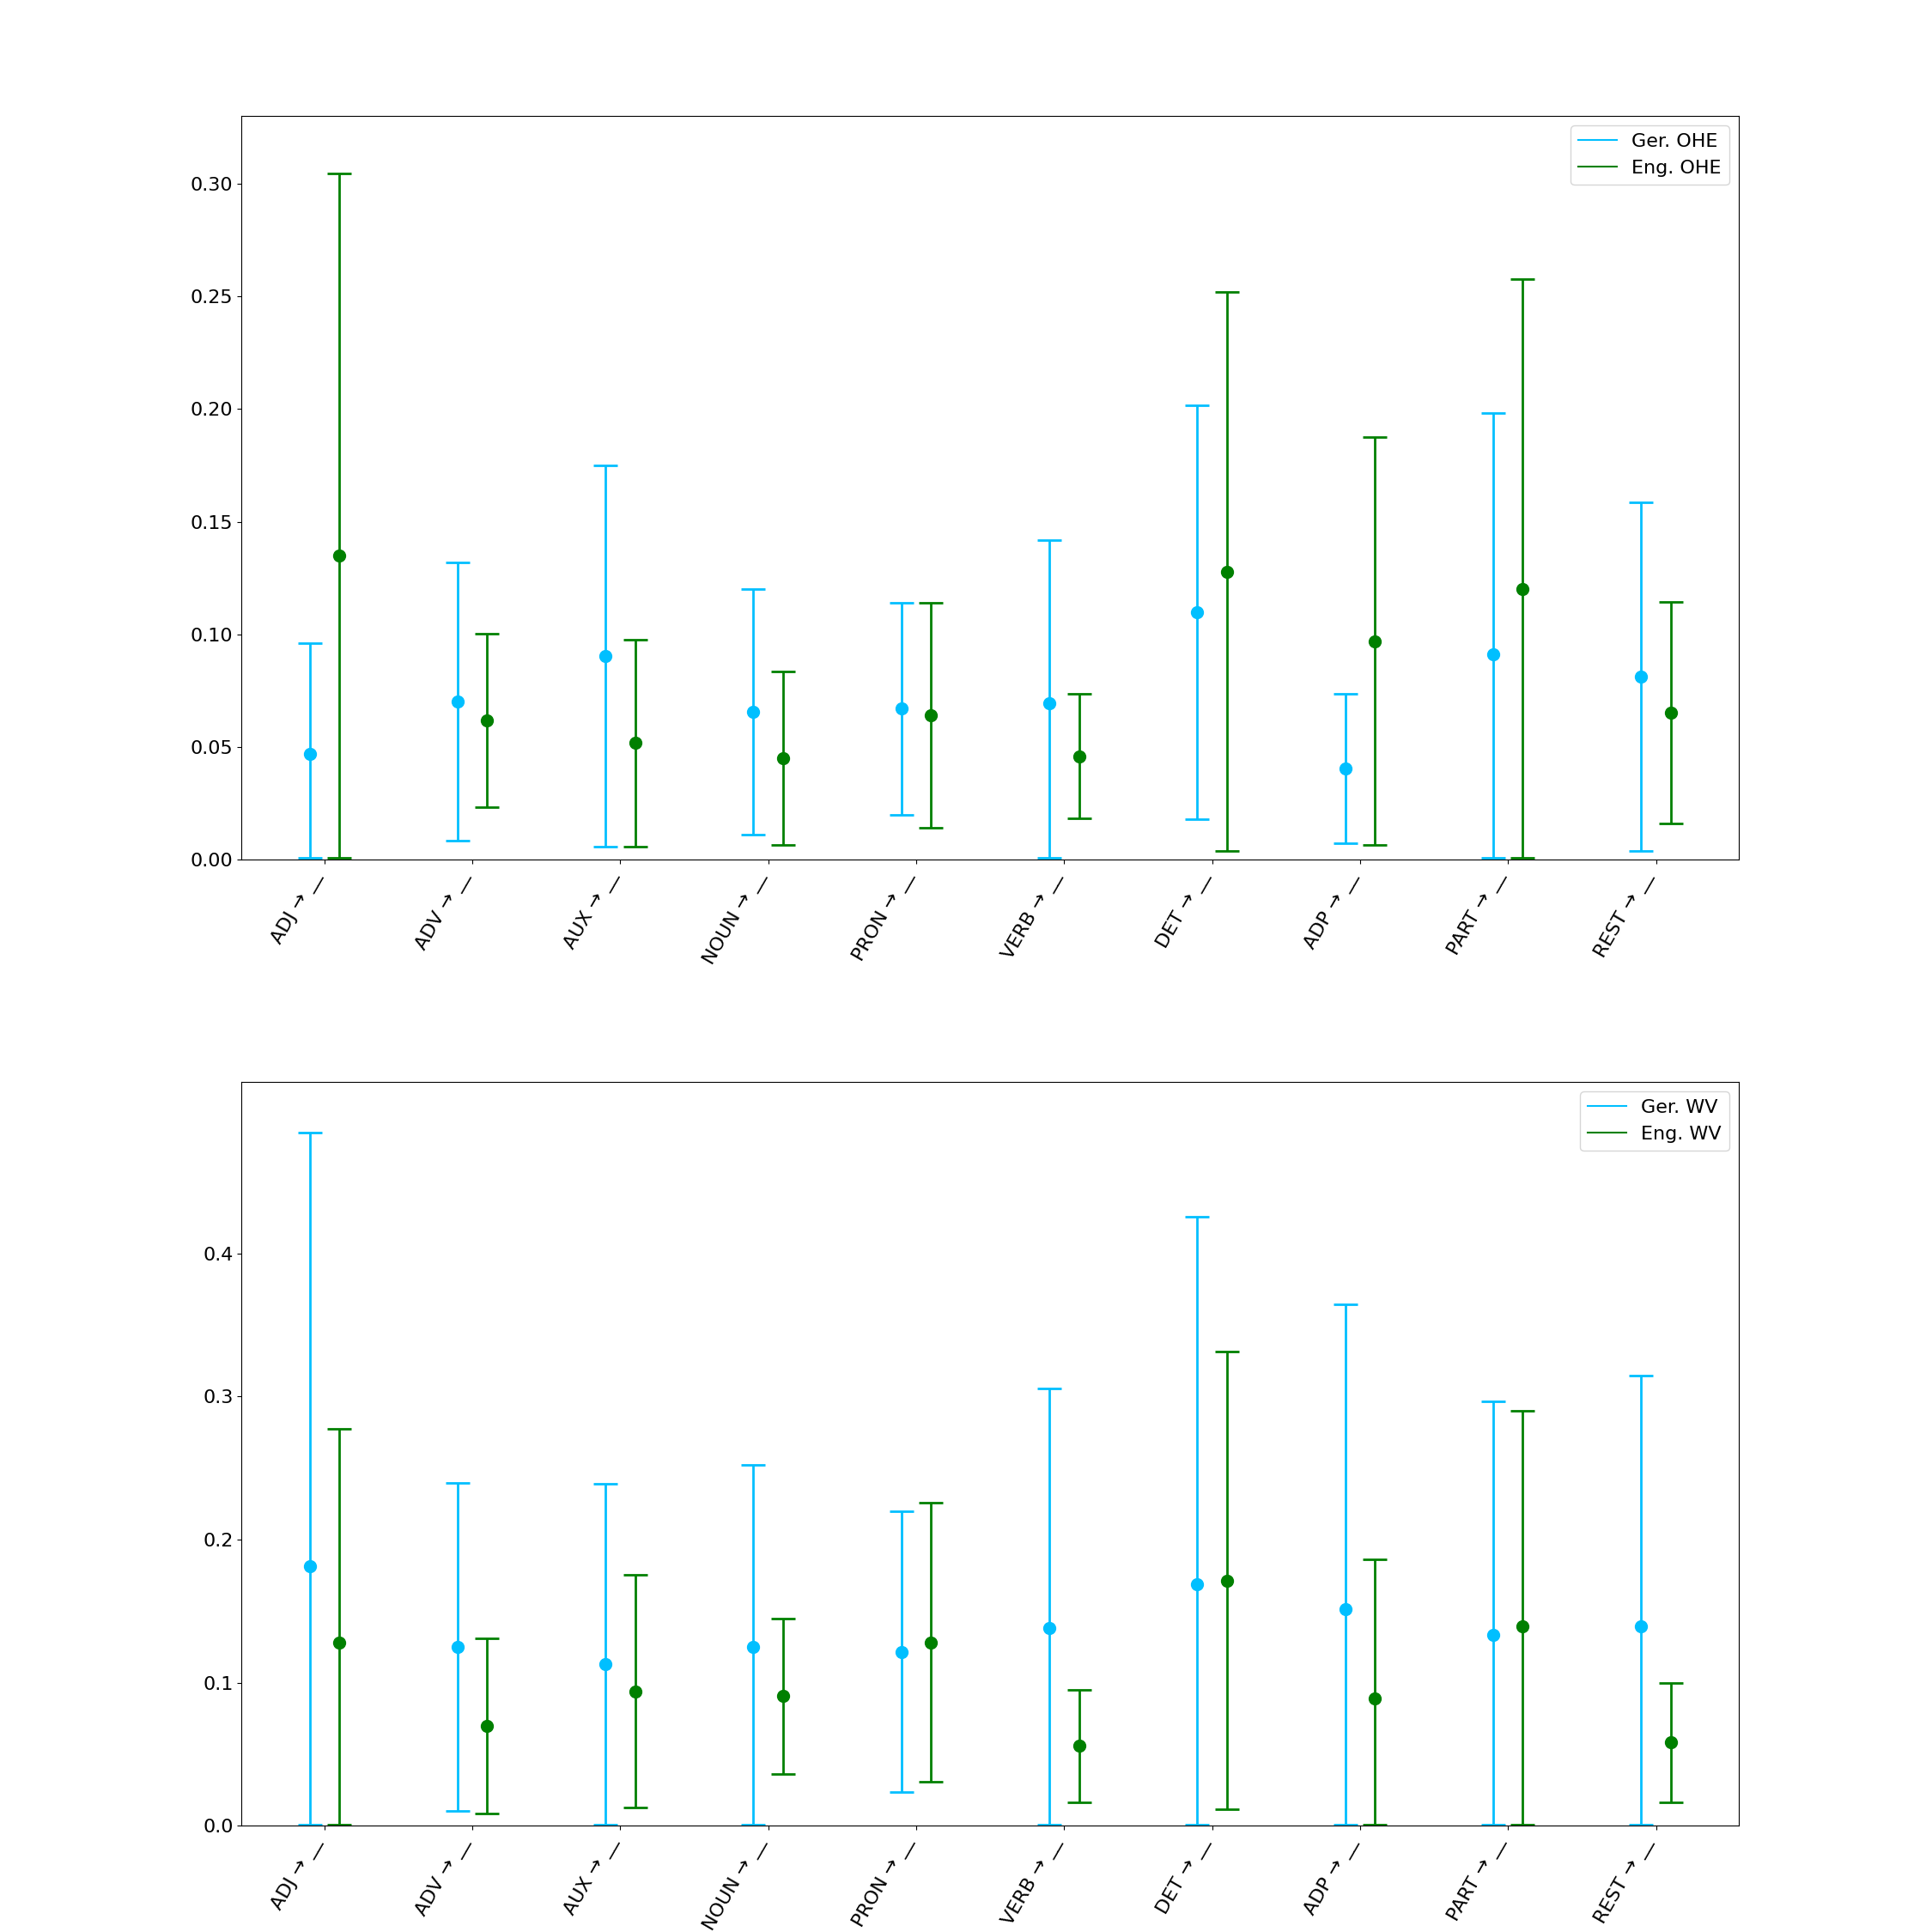
\includegraphics[scale=0.325, center]{code/error_com.png}
	\caption{Mean and standard deviation of the configurations \wrt to the ground truth \ie the difference between the ground truth matrix and the prediction matrix was used for the row wise calculations (matrices depicted in \figref{\ref{fig: avg model gt w2v de en}}). Clearly visible that \onehot{} models (OHE) outperform word vector versions (WV). Both, mean and standard deviation, are lower. Because a difference is assessed, smaller means are better.}
	\label{fig: rsme plots}
\end{figure}
All means are to some extent equal but the standard deviations differ. The free word order of German doesn't seem to be a problem because both models learn better than their English counterparts (\tabref{\ref{tab: avg model versions and metrics}}). There are some difficulties with adjectives (except for Ger. OHE), although they are tied to \texttt{NOUN} and \texttt{ADJ} (\figref{\ref{fig: barplot det adp}}).

Sadly, the prepared visualizations \ie \figref{\ref{fig: rsme plots}} and \tabref{\ref{tab: avg model versions and metrics}}, lack the ability to grasp the full picture: The word vector configurations seem to work by checking the means for each \postag{}, but when inspecting the matrices as a whole as in \figref{\ref{fig: avg model gt w2v de en}}, it is apparent that they don't. Whereas using the english book, the model degenerates to the identical distribution and the german one contemplates \texttt{NOUN} as its personal $ 42 $.
%By checking the averaged means of \figref{\ref{fig: rsme plots}} in \tabref{\ref{tab: avg model versions and metrics}}, it is unexpected that the english word vector model has a far lower value and is closer to \onehot{} variant than to the german equivalent. An impression which can also gained by \figref{\ref{fig: rsme plots}}. Although not comparable by mere numbers but rather qualitatively the score should be located closer to the other word vector model as in \tabref{\ref{tab: text model versions and metrics}} because the model structure is the same. This anomaly can be explained by inspecting the transition matrix as a whole as in \figref{\ref{fig: transitionprobabilitymatrixt1df0}}. It more or less resembles an identical distribution.
%
%Therefore, the low value of the english \onehot{} model is explained by the identically distributed predictions in this row.
\begin{table}
	\centering
	\caption{Averaged means of the difference between prediction and ground truth. As expected, the word vector versions have higher scores than the \onehot{} counterpart. These values can't be used for a comparison with \tabref{\ref{tab: text model versions and metrics}} because the underlying metrics are different.}
	\begin{tabular}{lll}
		\toprule
		Version					& Mean in $ 10^{-2} $	& Standard deviation in $ 10^{-2} $ \\
		\midrule
		german, \onehot{} 		& $ 7.3 $				& $ 2.0 $ \\% 0.08200
		german, word vector		& $ 14.0 $				& $ 2.1 $ \\% 0.74139
		english, \onehot{}		& $ 8.1 $				& $ 3.3 $ \\% 0.10021
		english, word vector	& $ 10.2 $				& $ 3.6 $ \\% 0.77522
		\bottomrule
	\end{tabular}
	\label{tab: avg model versions and metrics}
\end{table}
%
%As expected, the word vector versions have higher scores than the \onehot{} counterpart. Again, the german training data reached the best value, which makes sense after checking \figref{\ref{fig: avg model ohe de en tpm} and \ref{fig: avg model w2v de en tpm}}. Due to the more flexible sentence structure this was unforeseeable. Although derived from the illustration the approaches using word vectors don't seem to learn anything. Despite being close to its \onehot{} counterpart, the english word vector version seem to approach an identical distribution, whereas training with german word vectors (\figref{\ref{fig: avg model w2v de en tpm}}) fails completely and concentrates on \texttt{NOUN} as its personal $ 42 $.
%
\begin{figure}
	\centering
		\subcaptionbox{German, ground truth of word class transitions.}{
			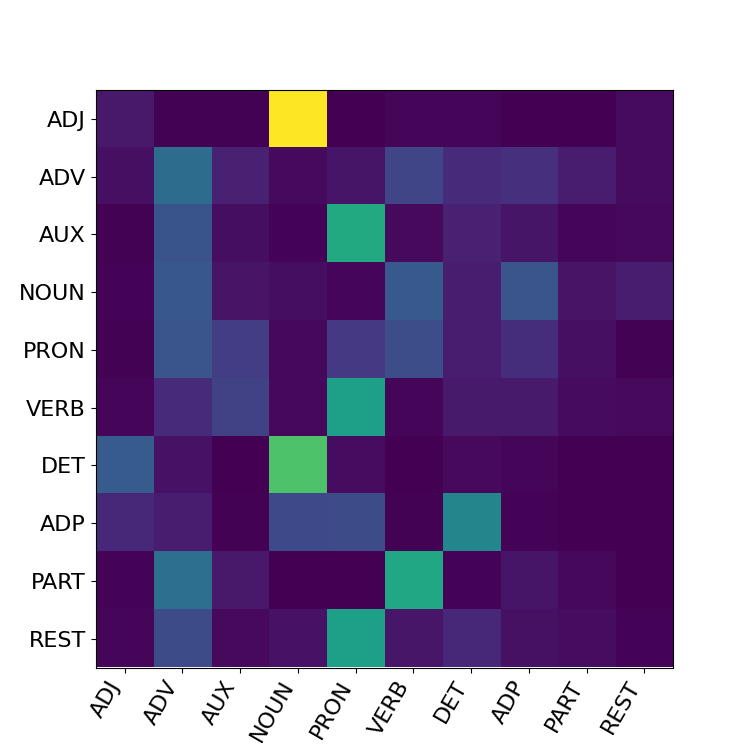
\includegraphics[height=\threerowpicheight]{Bilder/chapter4/average_models/ground_truths/D_200pages_1500T_tags.png}
		}
		\hspace*{1cm}
		\subcaptionbox{English, ground truth of word class transitions.}{
			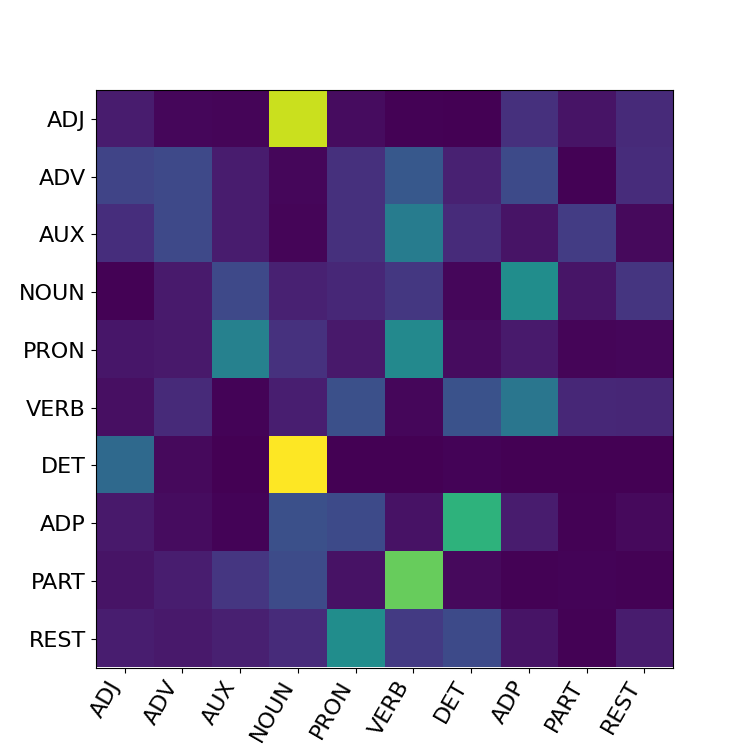
\includegraphics[height=\threerowpicheight]{Bilder/chapter4/average_models/ground_truths/J_200pages_1500T_tags.png}
		}
		\\
		\subcaptionbox{German, learned \gls{sr} using \onehot{s}.}{
			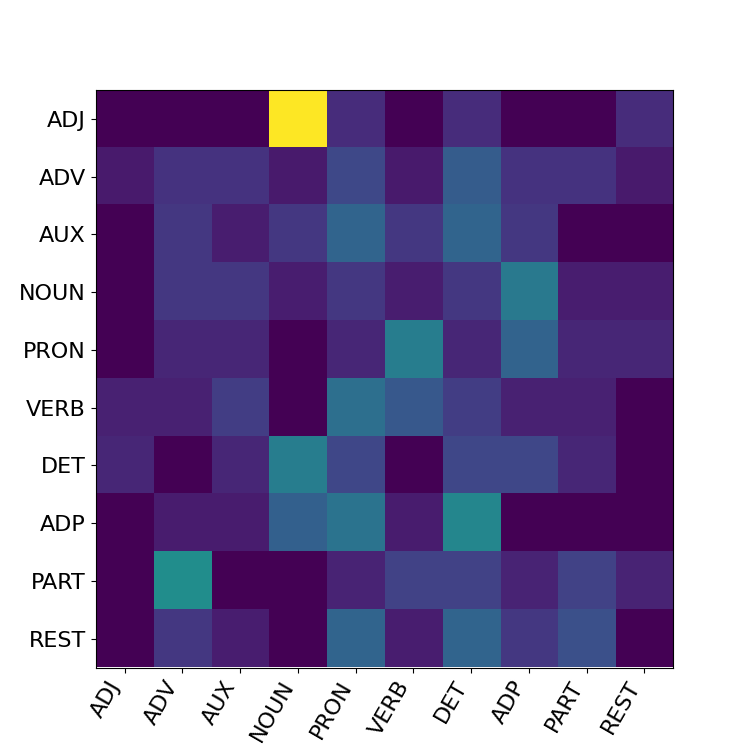
\includegraphics[height=\threerowpicheight]{Bilder/chapter4/average_models/plots/Avg_OHE_OHE_5000E_100BS_1L_1C_200P_1500T_D/_epochs-4000/Transition_Probability_Matrix;_t=1,_DF=0.5.png}
		}
		\hspace*{1cm}
		\subcaptionbox{English, learned \gls{sr} using \onehot{s}.}{
			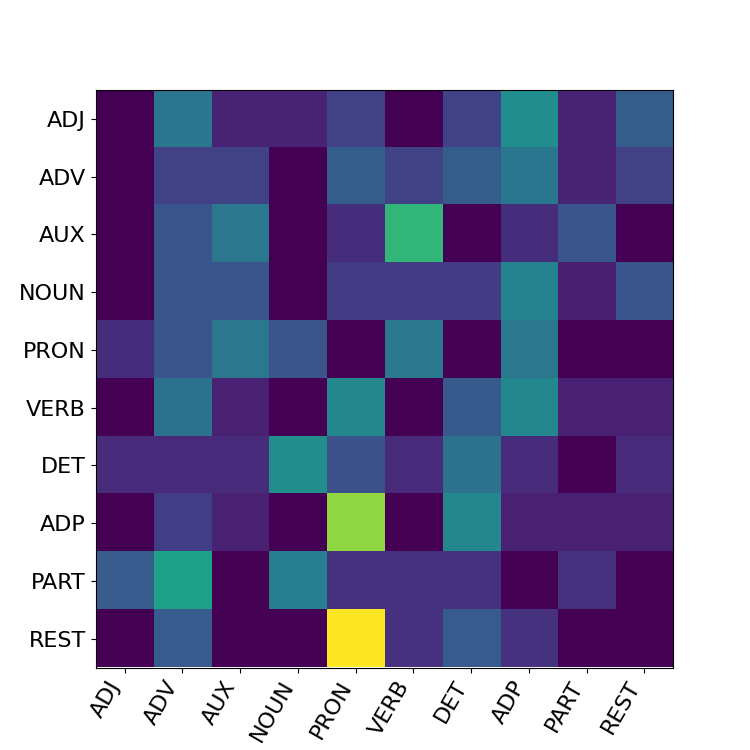
\includegraphics[height=\threerowpicheight]{Bilder/chapter4/average_models/plots/Avg_OHE_OHE_4000E_100BS_1L_1C_200P_1500T_J/Transition_Probability_Matrix;_t=1,_DF=0.5.png}
		}
		\\
		\subcaptionbox{German, learned \gls{sr} using word vectors.}{
			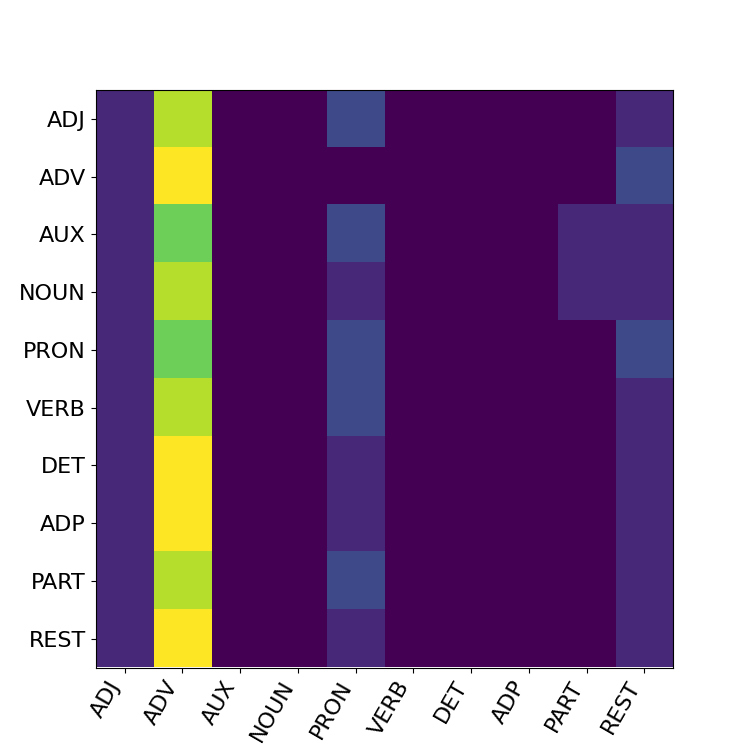
\includegraphics[height=\threerowpicheight]{Bilder/chapter4/average_models/plots/Avg_W2V_W2V_5000E_100BS_1L_1C_200P_1500T_D/_epochs-4000/Transition_Probability_Matrix;_t=1,_DF=0.5.png}
		}
		\hspace*{1cm}
		\subcaptionbox{English, learned \gls{sr} using word vectors.}{
			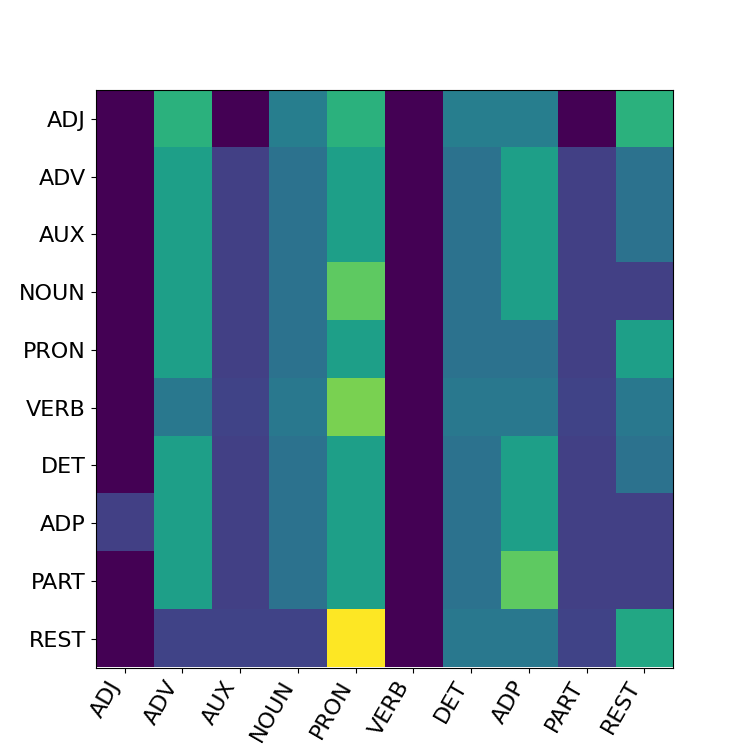
\includegraphics[height=\threerowpicheight]{Bilder/chapter4/average_models/plots/Avg_W2V_W2V_5000E_100BS_1L_1C_200P_1500T_J/_epochs-4000/Transition_Probability_Matrix;_t=1,_DF=0.5.png}
		}
	\caption{If word vectors are used for training the model has problems with both languages. When using German the predictions degenerate completely and will classify everything as \texttt{NOUN}. The outcome of precessing English is reversed: it is quite close to an identical distribution which equals mere guessing amidst the \postag{s}.}
	\label{fig: avg model gt w2v de en}
\end{figure}

%\begin{table}[H]
%	\centering
%	\caption{For each row of the learned matrices the \gls{rmse} was calculated according to the corresponding ground truth. The values mustn't be compared to \tabref{\ref{tab: text model versions and metrics}} since they were calculated differently. Last row show the average over the columns. Meaning of the acronyms: OHE = \onehot{}, WV = word vector.}
%	\begin{tabular}{lcccc}
%		\toprule
%		Transition & Ger. OHE & Ger. WV & Eng. OHE & Eng. WV \\
%		\midrule
%		\texttt{ADJ → \_\_\_}	& 0.15 & 0.79 & 0.48 & 0.44 \\
%		\texttt{ADV → \_\_\_}	& 0.20 & 0.38 & 0.16 & 0.21 \\
%		\texttt{AUX → \_\_\_}	& 0.27 & 0.38 & 0.15 & 0.28 \\
%		\texttt{NOUN → \_\_\_}	& 0.19 & 0.40 & 0.13 & 0.24 \\
%		\texttt{PRON → \_\_\_}	& 0.18 & 0.35 & 0.18 & 0.36 \\
%		\texttt{VERB → \_\_\_}	& 0.22 & 0.49 & 0.12 & 0.15 \\
%		\texttt{DET → \_\_\_}	& 0.32 & 0.69 & 0.40 & 0.52 \\
%		\texttt{ADP → \_\_\_}	& 0.12 & 0.58 & 0.30 & 0.29 \\
%		\texttt{PART → \_\_\_}	& 0.31 & 0.47 & 0.41 & 0.46 \\
%		\texttt{REST → \_\_\_}	& 0.25 & 0.50 & 0.19 & 0.16 \\
%		\hline
%		$ \varnothing $ & 0.21 & 0.50 & 0.25 & 0.31 \\
%		\bottomrule
%	\end{tabular}
%	\label{tab: avg model versions and metrics}
%\end{table}
